\chapter{Architektura rozwiązania}
\label{cha:architekturaRozwiazania}

%---------------------------------------------------------------------------

\section{Wprowadzenie do architektury}
\label{sec:wprowadzenieDoArchitektury}

Trzon rozwiązania stanowi plugin \textit{HowAreYou}. Plugin działa w~ramach frameworka \textit{AWARE}. Do wykorzystywania pluginu konieczna jest więc aplikacja kliencka \textit{AWARE}. Ponadto wewnątrz pluginu wkompilowana jest również biblioteka rdzeniowa \textit{AWARE-core}. Sam plugin działa więc jako niezależna aplikacja i jako osobna instancja \textit{AWARE}. Aplikacja kliencka służy jedynie do konfiguracji rozszerzenia.

\begin{figure}[H]
	\centering
	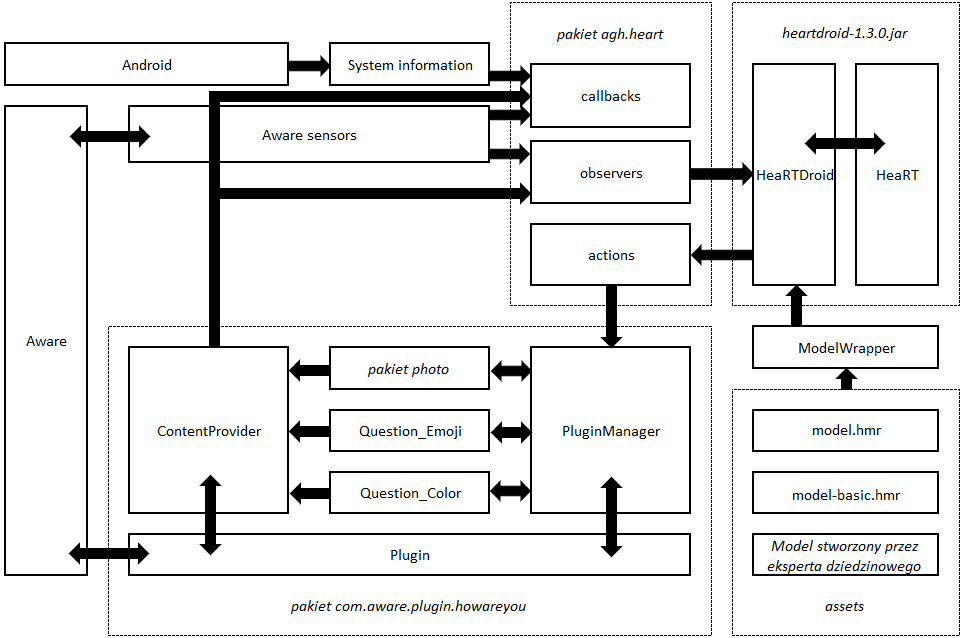
\includegraphics[scale=0.8]{rozdzial3/ArchitekturaSchemat.png}
	\caption{Schemat przedstawiający ogólną architekturę rozwiązania.}
\end{figure}

Wewnątrz pluginu wkompilowana jest również biblioteka silnika wnioskującego \textit{HeaRTDroid}. Dołączony pakiet \textit{agh.heart} (\textit{HeaRT-AWARE}) stanowi proxy pomiędzy zasadniczą częścią aplikacji a samym silnikiem. Plugin zawiera też kod \textit{XTT2} modeli wnioskujących dla silnika oraz implementuje rozwiązania, dzięki którym może komunikować się z~użytkownikiem, gromadzić dane i przesyłać te dane do wspólnej bazy. 

Powyższy schemat prezentuje najważniejsze składowe rozwiązania i zależności między nimi. Poza opisanymi tutaj elementami użytkownik ma do dyspozycji jeszcze aktywność ustawień, gdzie można konfigurować działanie oraz monitorować stan aplikacji.


%---------------------------------------------------------------------------

\section{Silnik wnioskujący}
\label{sec:silnikWnioskujacy}

\textit{HeaRTDroid} jest opartym na regułach silnikiem wnioskującym stworzonym z~myślą zarówno o urządzeniach mobilnych jak i rozwiązaniach desktopowych. Bazuje on na silniku wnioskującym \textit{HeaRT} i jest rozpowszechniany na licencji GNU GPL. Najważniejszymi cechami tego rozwiązania są\cite{heartdroid}:

\begin{itemize}
	\item wsparcie dla reprezentacji reguł \textit{XTT2} i dla języka HMR+, który je tekstowo reprezentuje.
	
	\item implementacja w~czystej Javie, co pozwala na integrację z~dowolnym innym kodem Javy, włączając to aplikacje mobilne dla systemu Android.
	
	\item integracja z~frameworkiem \textit{AWARE} zrealizowana w~formie rozszerzenia \textit{HeaRTDroid Plug-In}.
	
	\item mechanizm tzw. \textit{callbacks} oparty na refleksji w~języku Java, który pozwala na łatwą integrację z~innymi systemami.
	
	\item mechanizm zarządzania niepewnością oparty na algebrze współczynników pewności i podejściu probabilistycznym.
	
	\item różnorodne tryby wnioskowania i możliwość uruchomienia wnioskowania w~czasie rzeczywistym.
	
	\item oraz interaktywna powłoka linii komend \textit{HaQuNa}\cite{heartdroid}.
\end{itemize}

Na potrzeby pluginu \textit{HowAreYou} należało znaleźć rozwiązanie, które pozwoli na: 
\begin{itemize}
	\item swobodne zmiany modelu wnioskowania,
	
	\item możliwość uruchamiania silnika bezpośrednio na urządzeniu mobilnym z~systemem operacyjnym Android,
	
	\item łatwą współpracę z~frameworkiem \textit{AWARE}, służącym jako tzw. \textit{middleware} do akwizycji danych,
	
	\item możliwość uruchamiania wnioskowania bezpośrednio, gdy zmieni się jeden z~zewnętrznych czynników.
\end{itemize}

Stąd silnik \textit{HeaRTDroid} stał się oczywistym rozwiązaniem, jako że spełnia wszystkie powyższe założenia.

%---------------------------------------------------------------------------

\section{Model HMR}
\label{sec:modelHmr}

Plugin \textit{HowAreYou} został stworzony w~ten sposób, że wszystkie reguły wnioskujące silnika \textit{HeaRTDroid} mieszczą się poza kodem źródłowym aplikacji. W strukturze projektu \textit{Android Studio} pliki dodatkowe umieszcza się zazwyczaj w~katalogu \textit{assets} - tak jest rownież z~plikiem \textit{model.hmr}, który zawiera szczegółowy opis reguł w~języku zrozumiałym dla silnika wnioskującego.

%---------------------------------------------------------------------------

\section{Framework \textit{AWARE}}
\label{sec:frameworkAware}

Framework \textit{AWARE} to zaawansowane narzędzie pozwalające na gromadzenie, współdzielenie i wykorzystywanie szeroko pojętego mobilnego kontekstu. Umożliwia odczyt danych z~różnego rodzaju sensorów, filtrację i transfer do zdalnego serwera. Informacje kontekstowe przechowywane są w~przejrzystej strukturze bazy banych SQLite. 

\textit{AWARE} stanowi skuteczne oprogramowanie pośredniczące (ang. \textit{middleware}) umieszczone architektonicznie pomiędzy fizycznym sensorem a aplikacją użytkownika. Jednak jego głównym atutem jest możliwość realizacji pluginów -- czyli rozszerzeń, dodatków -- tworzonych przez niezależnych twórców bez ingerencji w~kod źródłowy aplikacji klienta czy rdzenia frameworku\cite{AwareFramework}. 


%---------------------------------------------------------------------------

\section{Pakiet \textit{HeaRT-AWARE}}
\label{sec:pakietHeartAware}

Jedną z~pierwszych kwestii, jakie trzeba było poruszyć na etapie projektowania rozwiązania, była kwestia zintegrowania ze sobą frameworka \textit{AWARE} i silnika wnioskującego \textit{HeaRTDroid}. Zdecydowano się tutaj skorzystać z~istniejącego rozwiązania, jakim jest plugin \textit{HeaRT-AWARE}. Aplikacja była realizowana przez Marka Wawrzosa na Katedrze Informatyki Stosowanej, a kod źródłowy został udostępniony studentom w~ramach platformy AI WIKI\cite{heartaware}.

Struktura projektu opiera się tutaj na dwóch pakietach: \textit{agh.heart} -- realizującym interackcje pluginu z~silnikiem wnioskującym i \textit{com.aware.plugin.template} -- realizującym standardową strukturę i standardowe zadania rozszerzenia \textit{AWARE}. W \textit{HowAreYou} zdecydowano się zrezygnować z~tej drugiej części, jako, że dysponowano już innym pakietem \textit{com.aware.plugin.howareyou}. Za to kluczową rolę w~realizacji aplikacji odegrał pakiet pierwszy, stanowiąc trzon proxy pomiędzy \textit{HeaRTDroid}em a \textit{AWARE}.

Na pakiet \textit{agh.heart} składają się następujące elementy:
\begin{itemize}
	\item \textit{actions} -- zestaw akcji, które mogą być podjęte (uruchomione) przez silnik regułowy (czyli \textit{de facto} mogą być wynikiem wnioskowania).
	
	\item \textit{callbacks} -- zestaw wywołań, które pozwalają mechanizmom wnioskującym na odwołanie się do parametrów zewnętrzych na przykład poprzez dostęp do baz danych pluginu, baz danych sensorów, czy informacji systemowych udostępnianych przez pakiety systemu Android.
	
	\item \textit{model} -- zestaw narzędzi pozwalających na wczytanie i obsługę modelu HMR. W pierwotnym rozwiązaniu model wczytywany był ze statycznego pola typu String. Na etapie projektowania zdecydowano się na zastąpienie statycznego wykorzystania modelu wyborem dynamicznym.
	
	\item \textit{observers} -- zestaw tzw. \textit{BroadcastReceivers}, które odpowiadają za uruchomienie wnioskowania w~chwili, gdy zostanie spełniony konkretny warunek.
	
	\item oraz klasa \textit{HeaRTService.java} odpowiedzialna za planowanie wnioskowania. Dzięki temu rozwiązaniu poszczególne zadania wnioskujące nie są uruchamiane równocześnie\cite{heartaware}.
\end{itemize}

Powyższe rozwiązanie zostało w~ramach niniejszej pracy znacznie rozbudowane przede wszystkim poprzez zaimplementowanie dodatkowych \textit{actions}, \textit{callbacks} i \textit{observers}.


%---------------------------------------------------------------------------

\section{Pakiet \textit{HowAreYou}}
\label{sec:pakietHowAreYou}


\subsection{Plugin \textit{AWARE}}

Plugin \textit{AWARE} działa na takiej zasadzie jak sensor \textit{AWARE} -- gromadzi dane. Może to jednak robić w~sposób bardziej inteligentny niż domyślnie zaimplementowane sensory -- wykorzystując dodatkowe informacje z~innych sensorów, filtrację informacji, czy akwizycję danych tylko w~konkretnych momentach. Może też łączyć w~sobie działanie wielu różnych źródeł informacji. Aby uniknąć nieoczekiwanych sytuacji, przy projektowaniu i implementacji rozszerzenia należy trzymać się struktury projektu wyznaczonej przez deweloperów \textit{AWARE}:

\begin{itemize}
	\item \textit{Syncadapter} -- usługa odpowiedzialna za synchronizację lokalnej bazy SQLite ze zdalnym serwerem.
	
	\item \textit{ContextCard} -- widok pluginu w~aplikacji klienta \textit{AWARE}. Pozwala użytkownikowi obserwować pracę pluginu.
	
	\item \textit{Plugin} -- klasa zarządzająca pozwoleniami systemu Android oraz wykorzystywanymi sensorami frameworka AWARE.
	
	\item \textit{ContentProvider} -- klasa zarządzająca bazami danych. Umożliwia inicjalizację tablic i wypełnianie ich danymi.
	
	\item \textit{Settings} -- klasa ustawień charakterystycznych dla danego pluginu. Z jej pomocą użytkownik może spersonalizować działanie aplikacji.
\end{itemize}

Twórcy rdzenia frameworka proponują, by komunikacja pomiędzy poszczególnymi elementami aplikacji odbywała się w~formie broadcastu. Realizacja pozostałych pakietów i klas pozostawiona jest w~gestii deweloperów\cite{AwareFramework}. 


\subsection{Dialog z~użytkownikiem}

Jednym z~najrzetelniejszych źródeł wiedzy o użytkowniku urządzenia mobilnego jest on sam. Dlaczegoby więc nie wykożystać tej wiedzy i nie zapytać go ,,Jak się czujesz?''. Należy tu jednak uważać, aby nie przekroczyć granicy, która jest bardzo cienka. Statystyczny Kowalski niemal natychmiast zrezygnuje z~naszego oprogramowania, jeżeli zacznie ono mu się naprzykrzać. Stąd konieczność pytania jedynie w~uzasadnionych przypadkach -- na przykład kiedy inne źródła danych kontekstowych wskażą, że nastrój właściciela telefonu uległ w~ostatnim czasie zmianie. W projekcie wykorzystany jest zestaw reguł do decydowania, kiedy należy pytać o emocje.

W pluginie zaimplementowano dwa sposoby odpytywania użytkownika o nastrój: oparty o \textit{emoji} i oparty o kolory. W obecnej realizacji właściciel telefonu komórkowego w~ustawieniach aplikacji ma możliwość wyboru: żadnego, jednego lub obu sposobów.

W przypadku pytania o emocje zadaniem użytkownika po wyświetleniu ekranu jest kliknięcie odpowiedniej emotikony z~napisem. Jeżeli żadna ikona nie zostanie wybrana, ekran zniknie po kilku sekundach.

Dodatkowo wprowadzono bardziej psychologiczne pytanie -- pytanie o kolory. W tym drugim przypadku zadaniem użytkownika po wyświetleniu ekranu jest wybór odpowiedniego koloru. W tym celu zaimplementowano mechanizm wyboru koloru. Jeżeli żaden kolor nie zostanie wybrany, ekran zniknie po kilku sekundach. Jeżeli zostanie wybrany, użytkownik może zatwierdzić wybór przyciskiem, zmienić wybór lub zaczekać - wówczas ekran zniknie i zostanie zapisana ostatnio wybrana odpowiedź.

\begin{figure}[H]
	\centering
	\begin{subfigure}{0.35\textwidth}
		\centering
		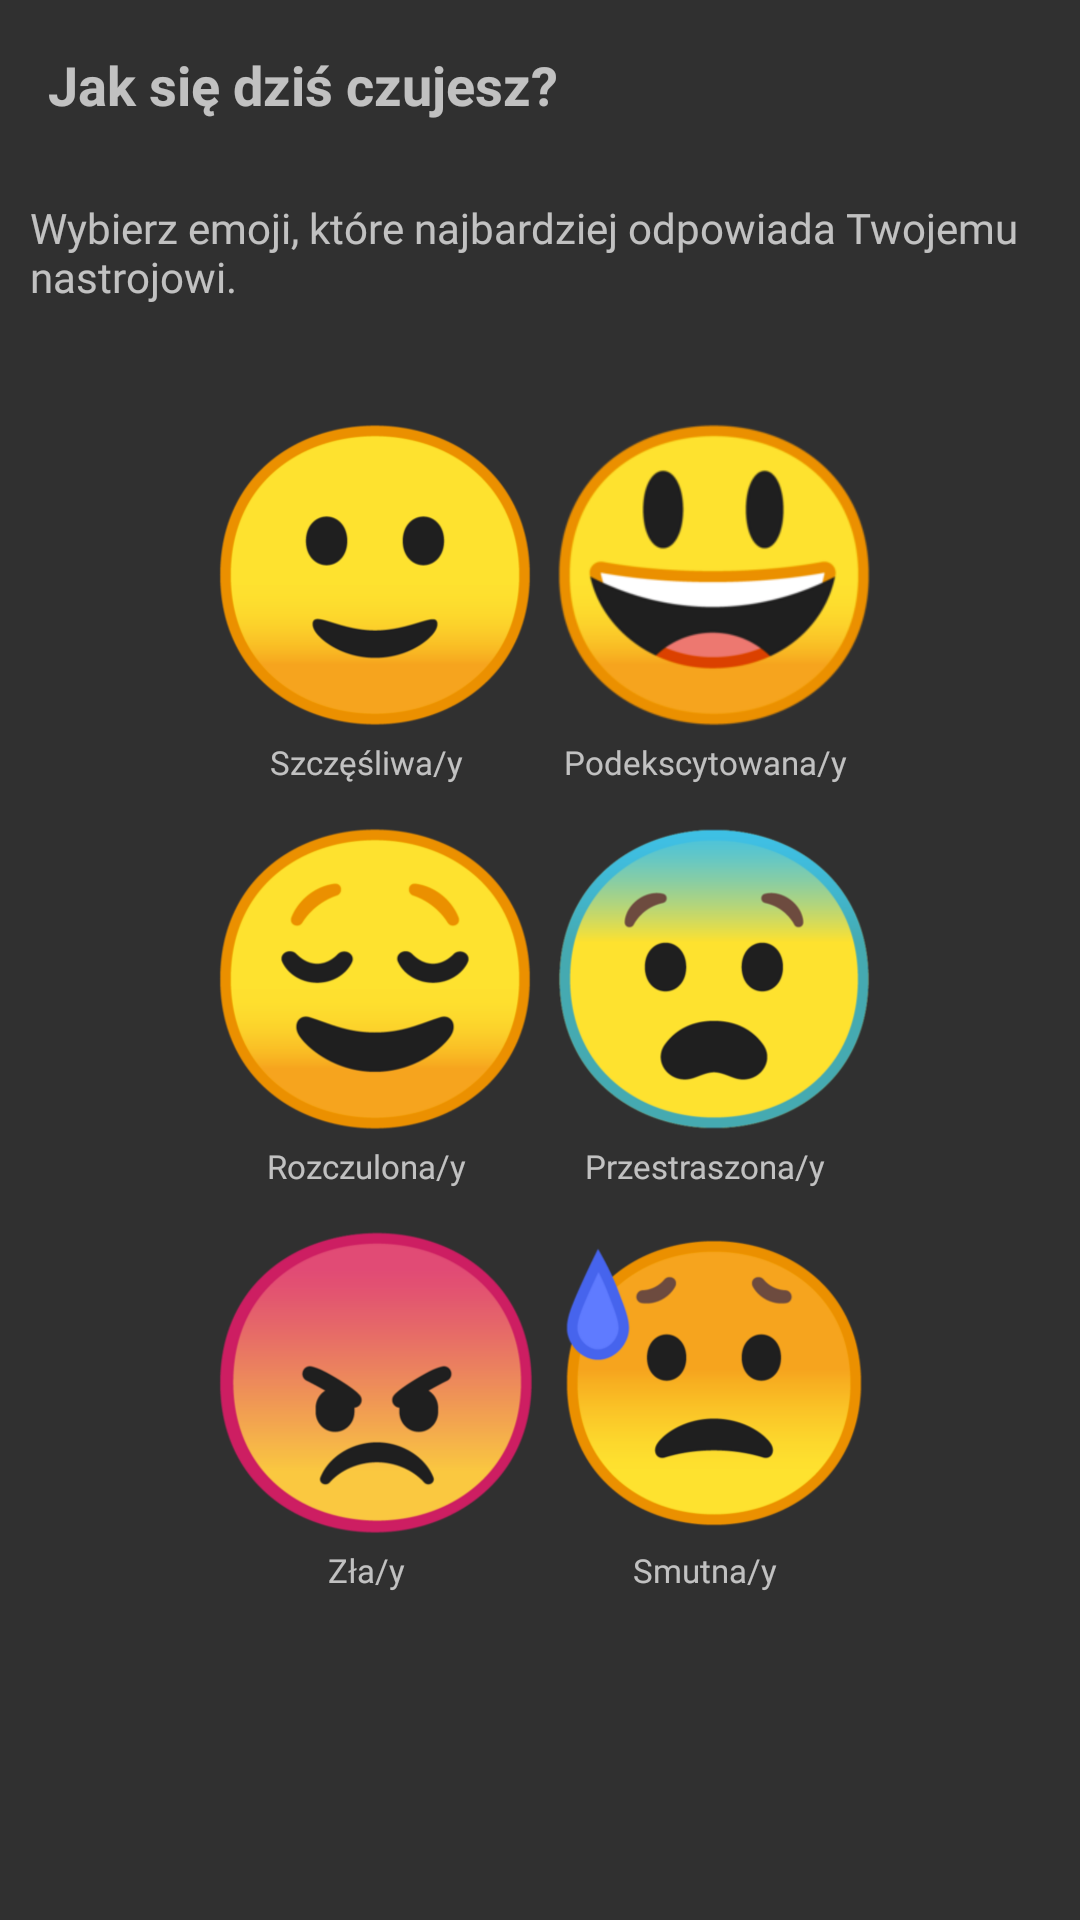
\includegraphics[scale=0.13]{rozdzial3/screen-emoji.png}
		\subcaption{\label{subfigure_a}}
	\end{subfigure}
	\begin{subfigure}{0.35\textwidth}
		\centering
		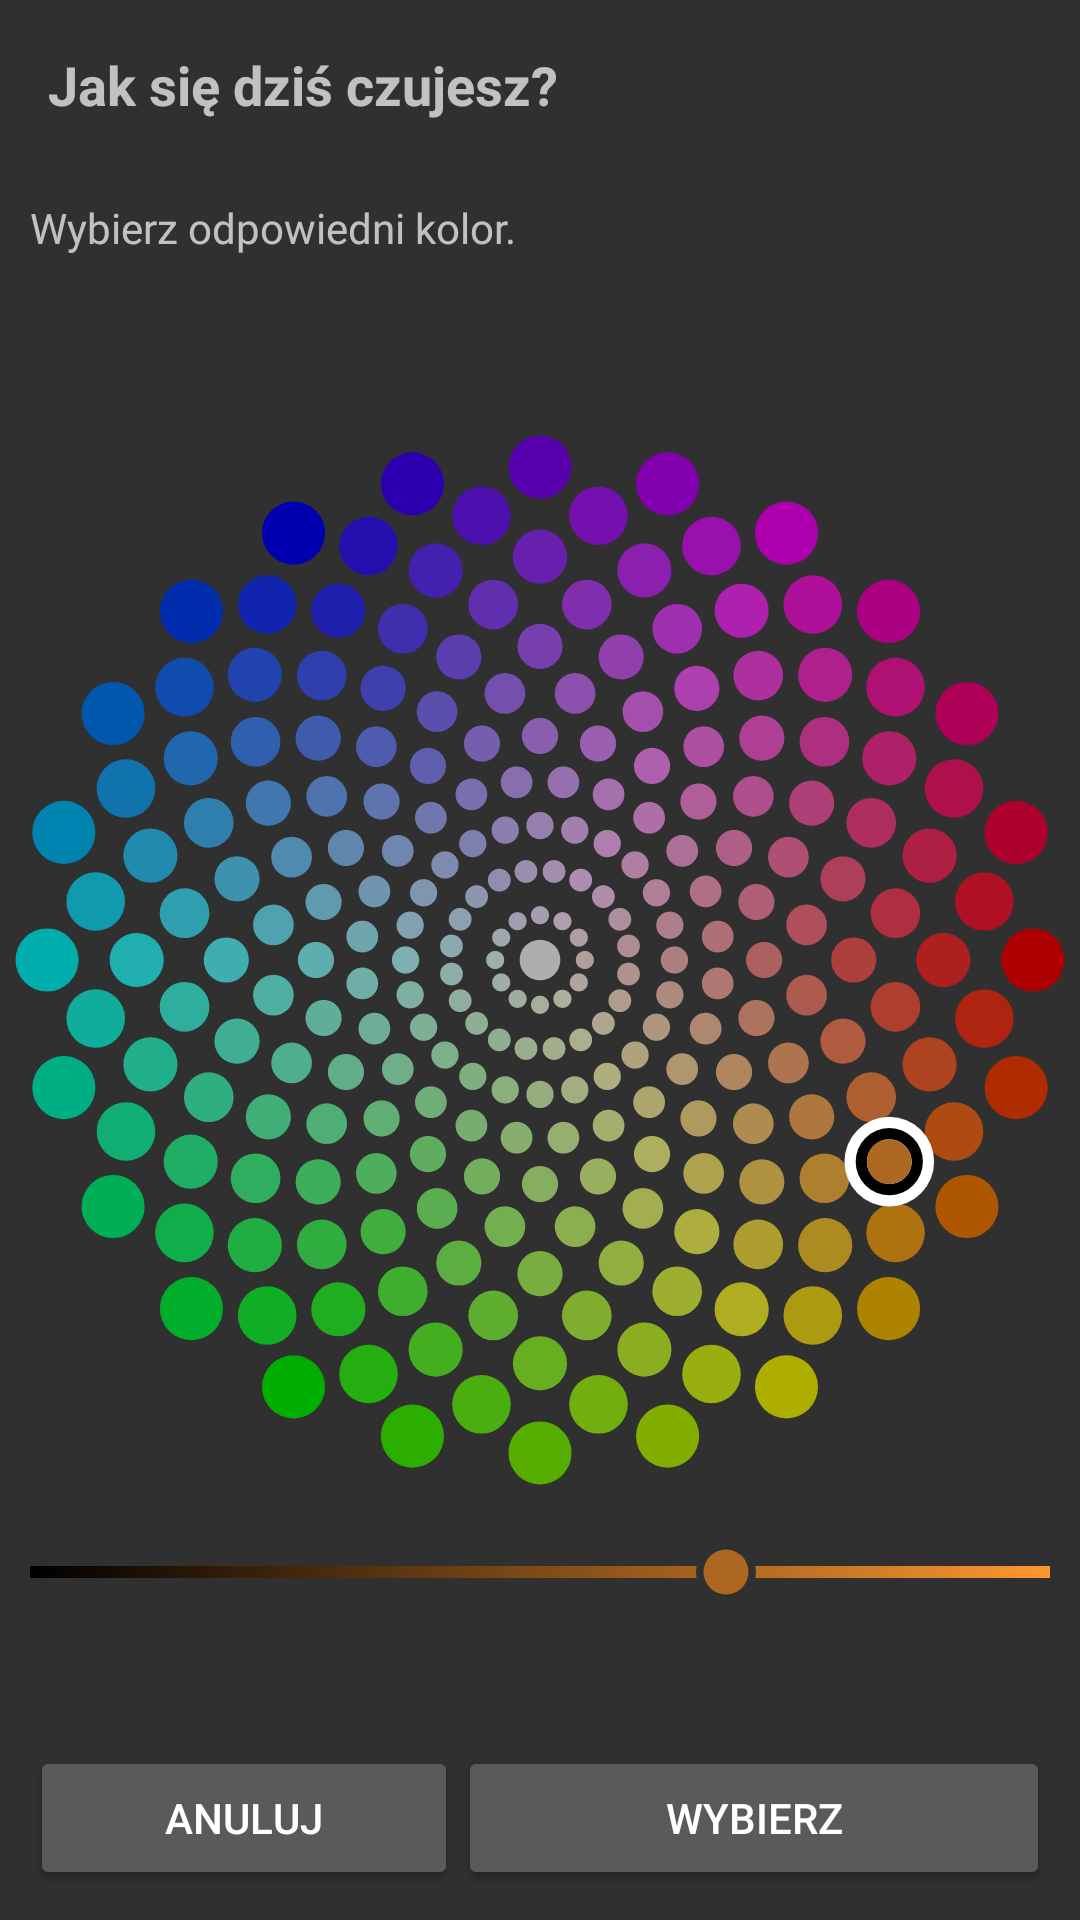
\includegraphics[scale=0.13]{rozdzial3/screen-color.png}
		\subcaption{\label{subfigure_b}}
	\end{subfigure}
	\caption{ Dialog z~użytkownikiem w~formie pytania o emocje (a) oraz pytania o kolory (b).}
\end{figure}


\subsection{Pakiet \textit{photo}}

W dwudziestym pierwszym wydaniu systemu Android, Google udostępniło deweloperom narzędzie, które pozwala kontrolować dostępne w~smartfonie aparaty – \textit{android.hardware.camera2} API. Zaimplementowany w~pluginie \textit{HowAreYou} pakiet \textit{photo} jest odpowiedzialny za wszytkie czynności potrzebne do wykonania zdjęcia ,,w tle'', to znaczy automatycznie, bez konieczności podglądu użytkownika, odpowiednim aparatem. Zdjęcia wykonywane są tylko i wyłącznie wtedy, gdy jest na to zgoda użytkownika.

\begin{figure}[H]
	\centering
	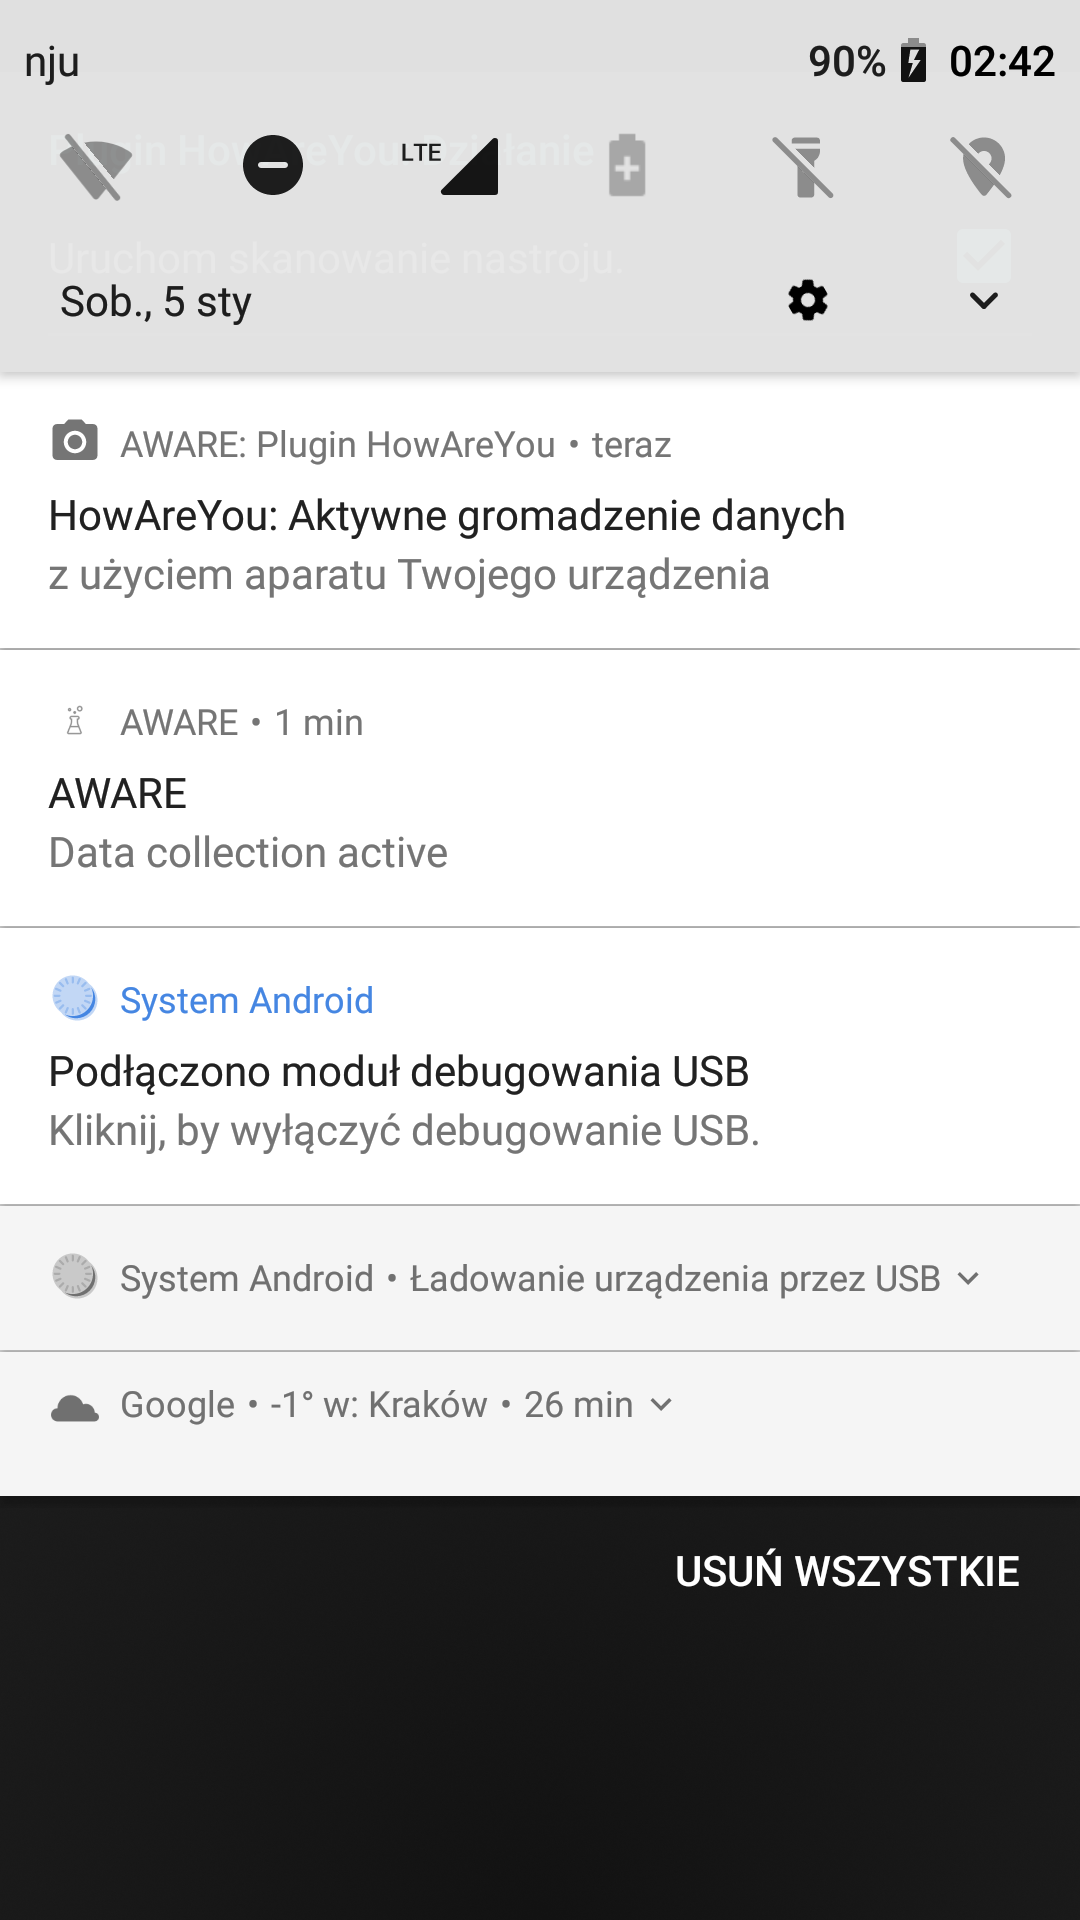
\includegraphics[scale=0.13]{rozdzial3/screen-background.png}
	\caption{Użytkownik może zdecydować, aby powiadomienie przypominało mu o możliwości rejestracji wizerunku.}
\end{figure}

Podobnie jak dialog z~użytkownikiem, rozpoznawanie emocji z~wykorzystaniem kamery telefonu zostało zrealizowane w~pluginie od zera -- wykorzystując doświadczenie zdobyte w~trakcie tworzenia aplikacji \textit{HowAreYou} i łącząc je z~możliwościami frameworka \textit{AWARE}. Poprawiono wykorzystanie \textit{camera2 API}. Zdjęcia są teraz wyraźne i odpowiednio naświetlone. Fotografie robione są w~tle, bez ingerencji w~działanie użytkownika. W przypadku niepowodzenia wykrycia emocji proces może być powtórzony zadaną ilość razy w~zadanym interwale.

Samo wykrywanie emocji składa się z~dwóch etapów. W pierwszym etapie wykorzystywany jest \textit{FaceDetector} Google. Z jego pomocą plugin sprawdza obecność twarzy w~kadrze zdjęciowym i dopiera najlepszą rotację zdjęcia dla dalszego procesowania. W dalszej części plik jest wysyłany do serwera \textit{MS Face API} gdzie następuje rozpoznanie emocji. Informacja zwrotna zostaje zapisana w~bazie \textit{SQLite}.


\subsection{Menu ustawień}


Aby uruchomić aktywność ustawień, w~aplikacji klienckiej \textit{AWARE} w~menu \textit{Plugins} należy wybrać \textit{HowAreYou}, a następnie \textit{Settings}. Po naciśnięciu przycisku oczom użytkownika ukaże się menu, za pomocą którego można konfigurować plugin. Z poziomu menu możliwe jest:

\begin{itemize}
	\item całkowite wyłączenie i ponowne włączenie pluginu \textit{HowAreYou}.
	
	\item włączenie/wyłączenie wykorzystania kamery. Ta opcja może być ważna dla osób, które cenią swoją prywatność. Dzięki niej mogą kontrolować, kiedy dokładnie wykonywane są fotografie.
	
	\item włączenie/wyłączenie wyświetlania przypomnienia, gdy kamera jest aktywna. Jeżeli użytkownik bierze udział w~krótkim badaniu, może nie być przyzwyczajony do tego, że jego kamera jest aktywna. Ikona aparatu na pasku powiadomień i powiadomienie po rozwinięciu górnego paska mogą mu o tym przypomnieć.
	
	\item włączenie/wyłączenie odpytywania użytkownika z~użyciem emotikon oraz kolorów. Odpytywanie można wyłączyć całkowicie. Można też zdecydować się na jedną z~dwóch dostępnych opcji.
	
	\item włączenie/wyłączenie trybu synchronizacji danych tylko przez wifi. Ilość danych do zsynchronizowania może być naprawdę niemała, dlatego została zaprojektowana taka opcja z~myślą o osobach, które nie dysponują dużym pakietem zbędnych gigabajtów.
	
	\begin{figure}[H]
		\centering
		\begin{subfigure}{0.35\textwidth}
			\centering
			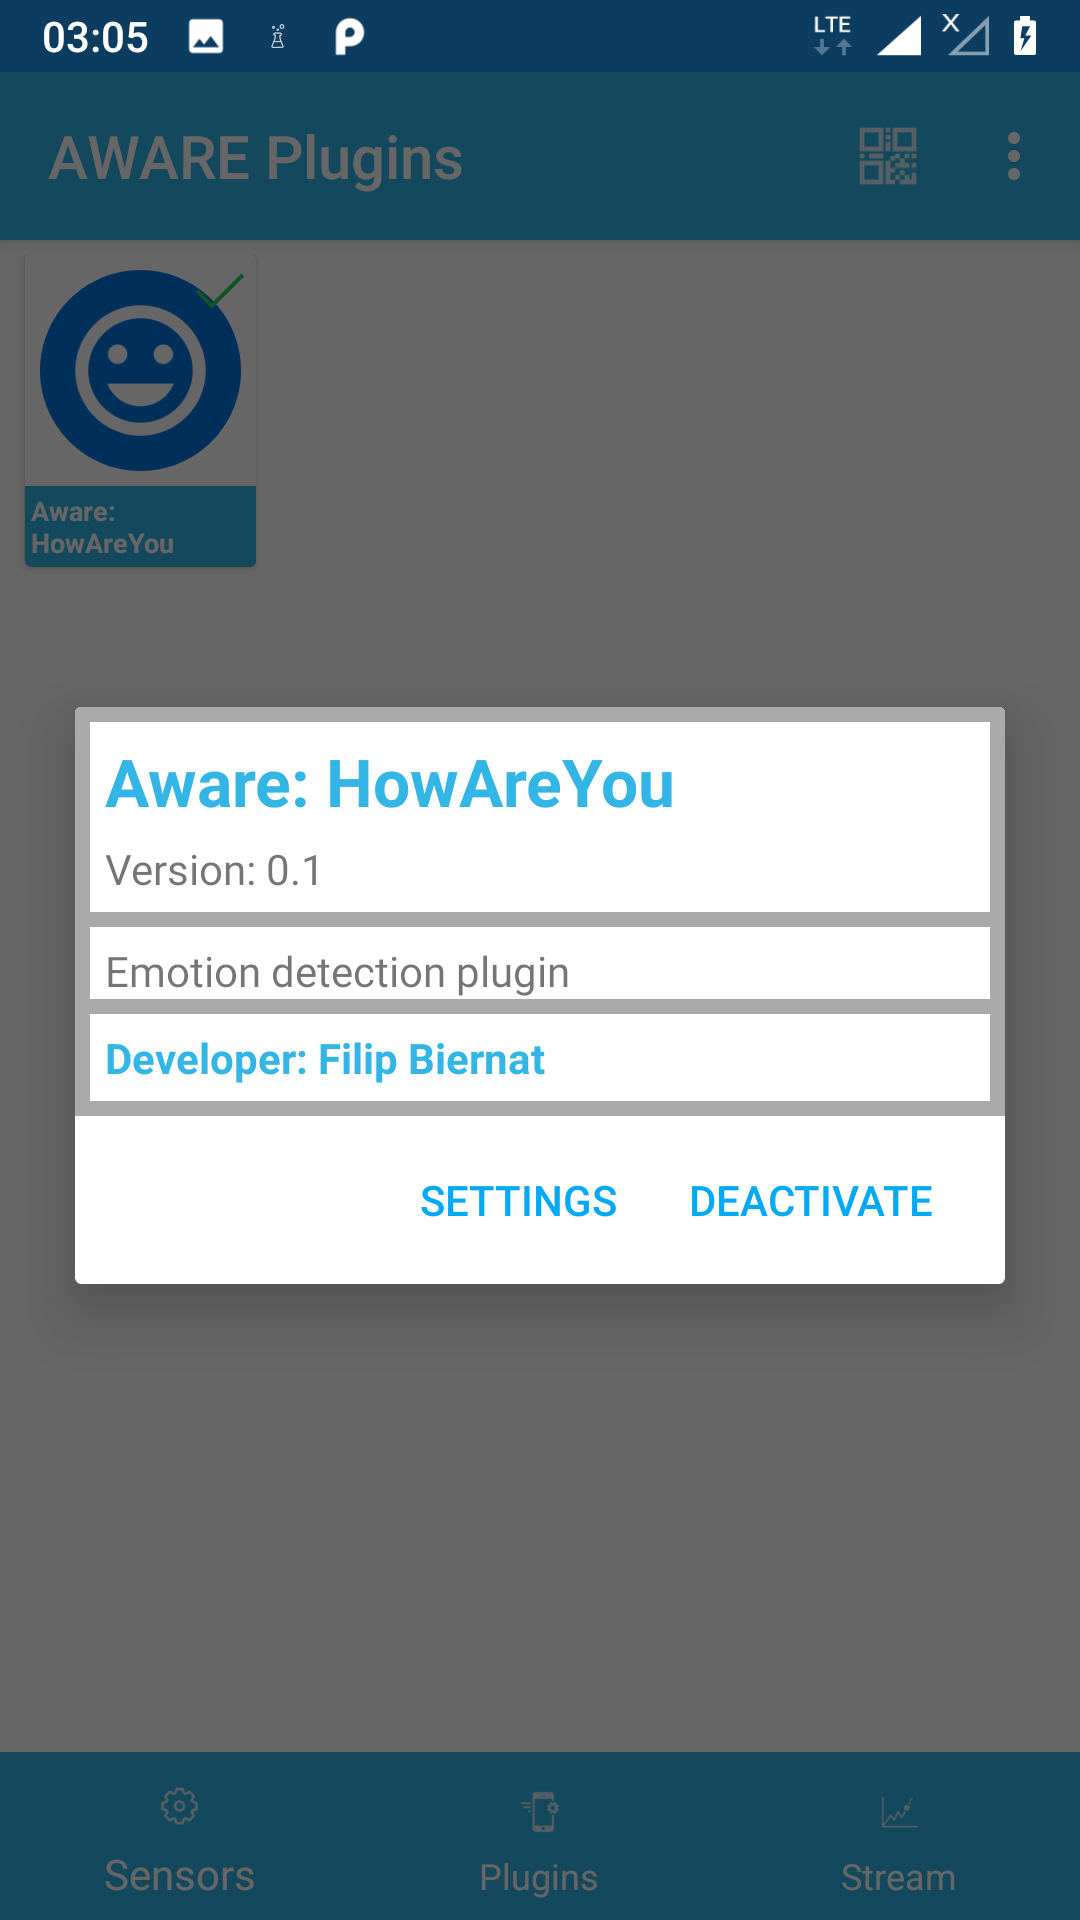
\includegraphics[scale=0.13]{rozdzial3/Ustawienia_uruchomienie.png}
			\subcaption{\label{subfigure_a}}
		\end{subfigure}
		\begin{subfigure}{0.35\textwidth}
			\centering
			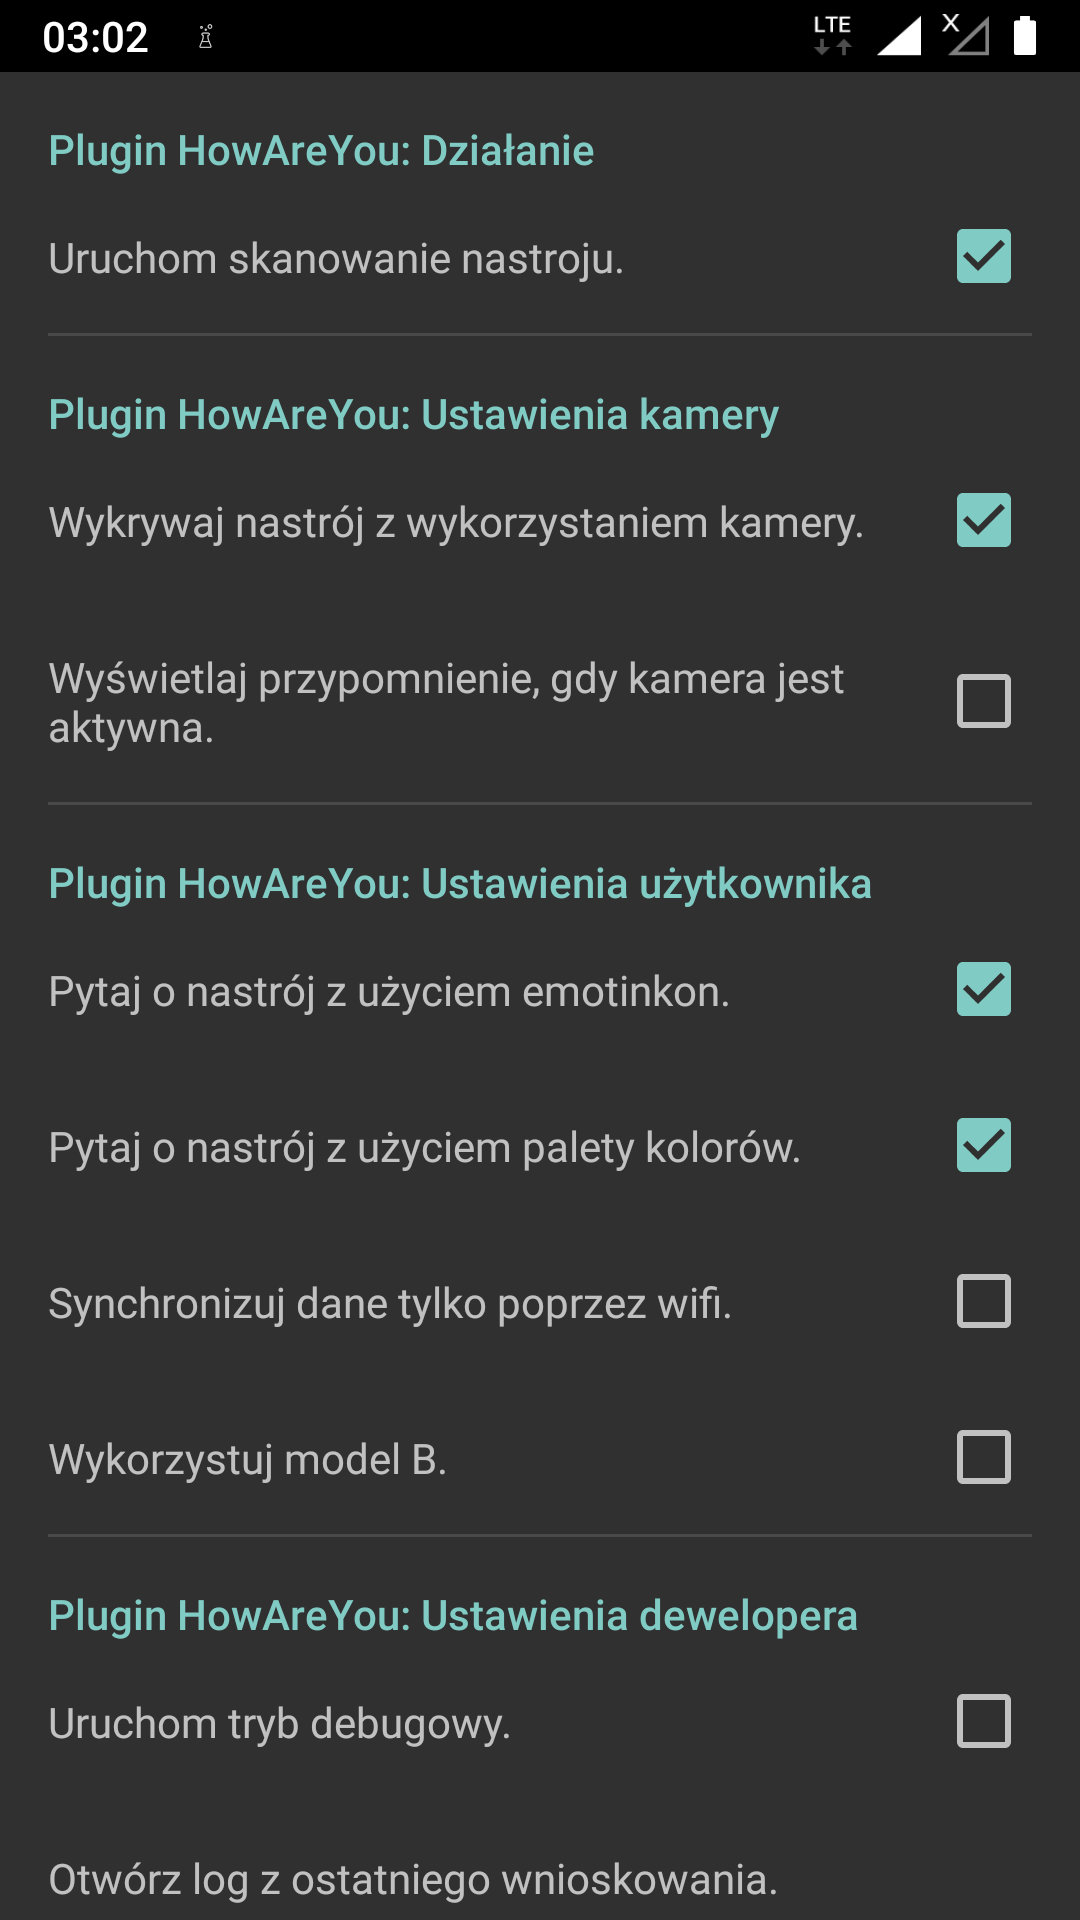
\includegraphics[scale=0.13]{rozdzial3/Ustawienia_cz1.png}
			\subcaption{\label{subfigure_b}}
		\end{subfigure}
		\caption{ Przejście do menu ustawień z~aplikacji klienckiej (a) oraz widok aktywności ustawień (b).}
	\end{figure}
	
	\item wybranie między modelem A (zaawansowany model HMR, \textit{patrz: rozdział 4}), a modelem B (wersja uproszczona modelu). Przy instalacji wersji A (\textit{patrz: dodatek A}), domyślnie wybrany jest model A, przy wersji B - model B.
	
	\item uruchomienie trybu debugowego. W trybie debugowym na ekranie urządzenia wyświetlają się w~formie wiadomości \textit{Toast} lub okna dialogowego dodatkowe informacje dotyczące działania algorytmów w~tle. Na dłuższą metę użytkowanie telefonu z~\textit{HowAreYou} w~trybie debugowym może być bardzo irytujące i dlatego jest niezalecane.
	
\end{itemize}

Z poziomu menu ustawień możemy też obserwować działanie aplikacji. Możliwe jest:

\begin{itemize}
	\item uruchomienie logu z~ostatniego wnioskowania. Taki log zawiera informacje, jakie zwraca silnik wnioskujący \textit{HeaRTDroid}. Dane są przetworzone z~użyciem specjalnego parsera, aby można je było analizować w~nieco bardziej przejrzystej formie.
	
	\item uruchomie logu aplikacji. Użytkownik może śledzić kolejne akcje tak, jakby to robił patrząc w~konsolę \textit{Logcat}. Widok umożliwia śledzenie aplikacji bez \textit{ADB}. Log samodzielnie się nie odświeża.
	
	\begin{figure}[H]
		\centering
		\begin{subfigure}{0.35\textwidth}
			\centering
			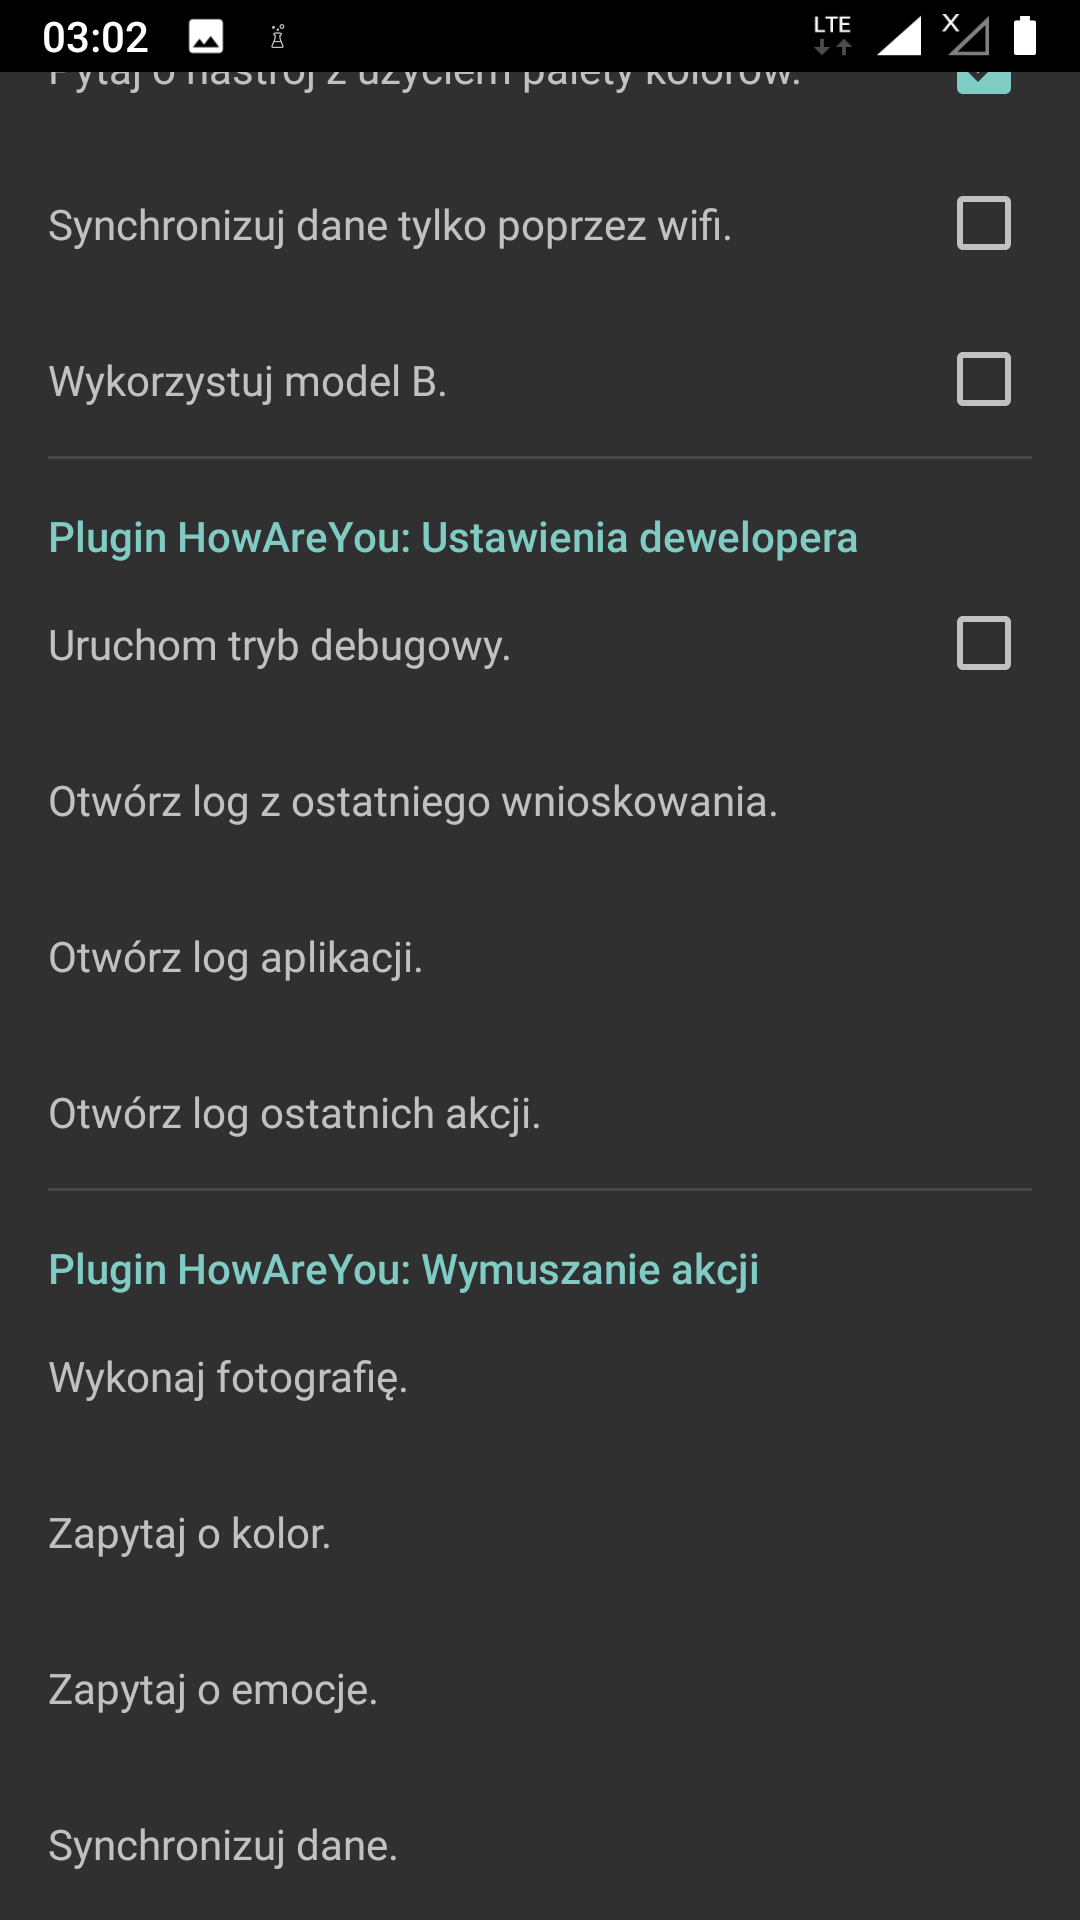
\includegraphics[scale=0.13]{rozdzial3/Ustawienia_cz2.png}
			\subcaption{\label{subfigure_a}}
		\end{subfigure}
		\begin{subfigure}{0.35\textwidth}
			\centering
			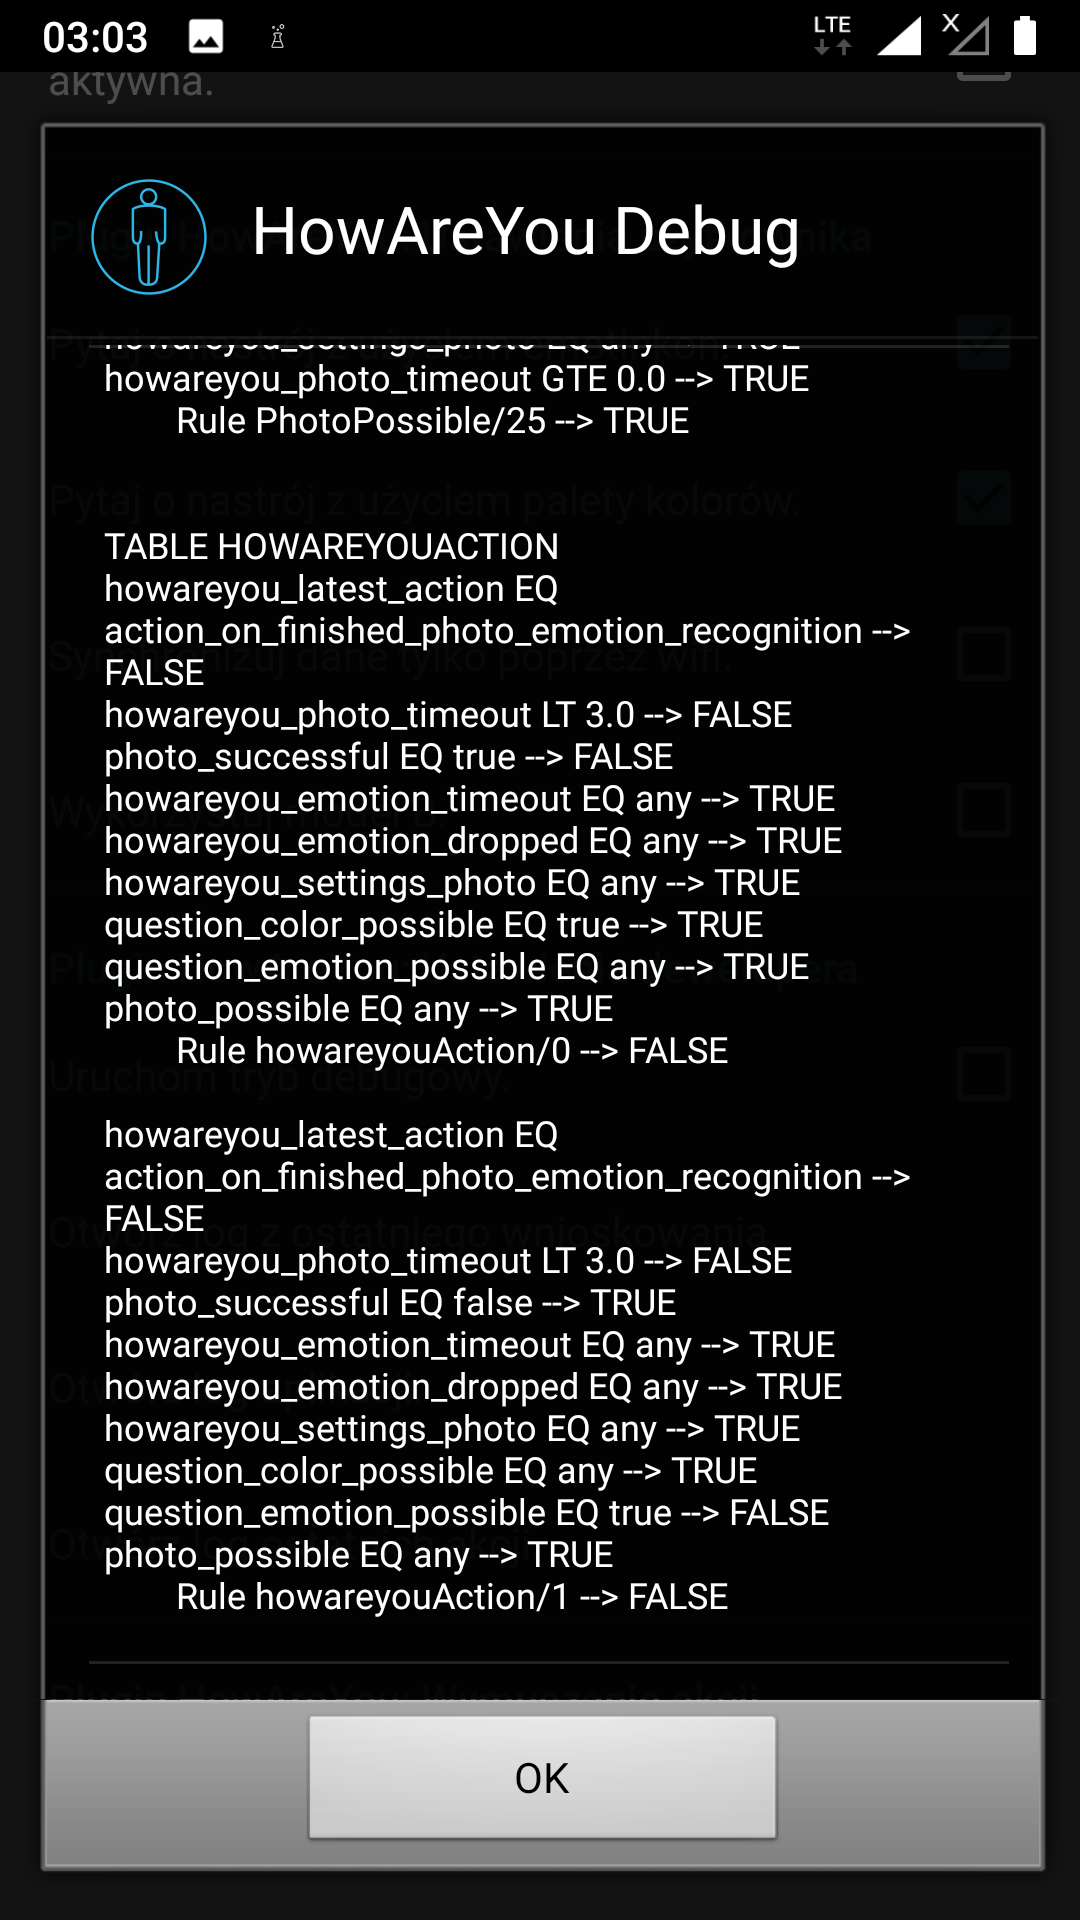
\includegraphics[scale=0.13]{rozdzial3/Ustawienia_logZWnioskowania.png}
			\subcaption{\label{subfigure_b}}
		\end{subfigure}
		\caption{ Widok dalszej części aktywności ustawień (a) oraz log z~ostatniego wnioskowania (b).}
	\end{figure}
	
	\item uruchomienie logu ostatnich akcji. Poza samą listą kolejnych akcji użytkownik ma do dyspozycji informację o znaku czasu ostatniej akcji każdego typu, o łącznej ilości akcji danego typu jaka została wykonana na urządzeniu, oraz o ilości akcji danego typu, która wykonała się w~ciągu ostatnich 24 godzin.
\end{itemize}

\begin{figure}[H]
	\centering
	\begin{subfigure}{0.35\textwidth}
		\centering
		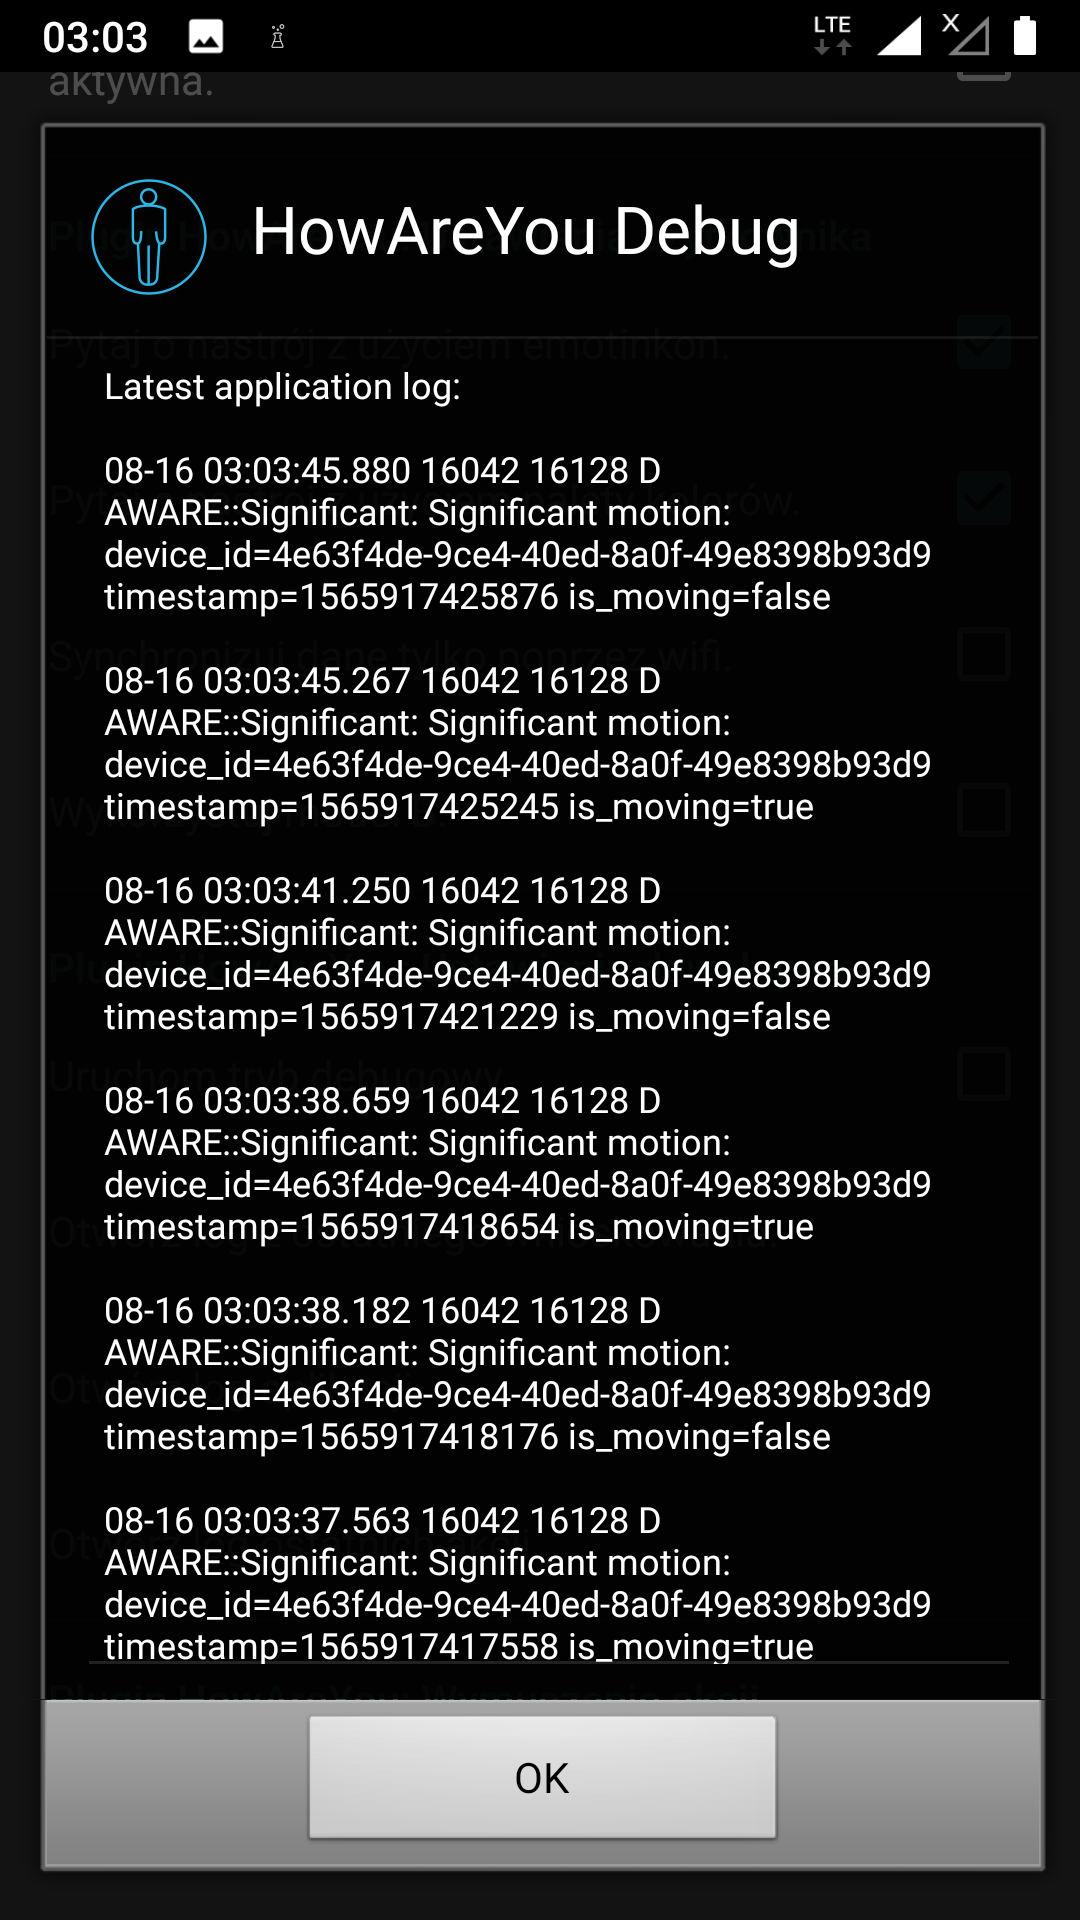
\includegraphics[scale=0.13]{rozdzial3/Ustawienia_logAplikacji.png}
		\subcaption{\label{subfigure_a}}
	\end{subfigure}
	\begin{subfigure}{0.35\textwidth}
		\centering
		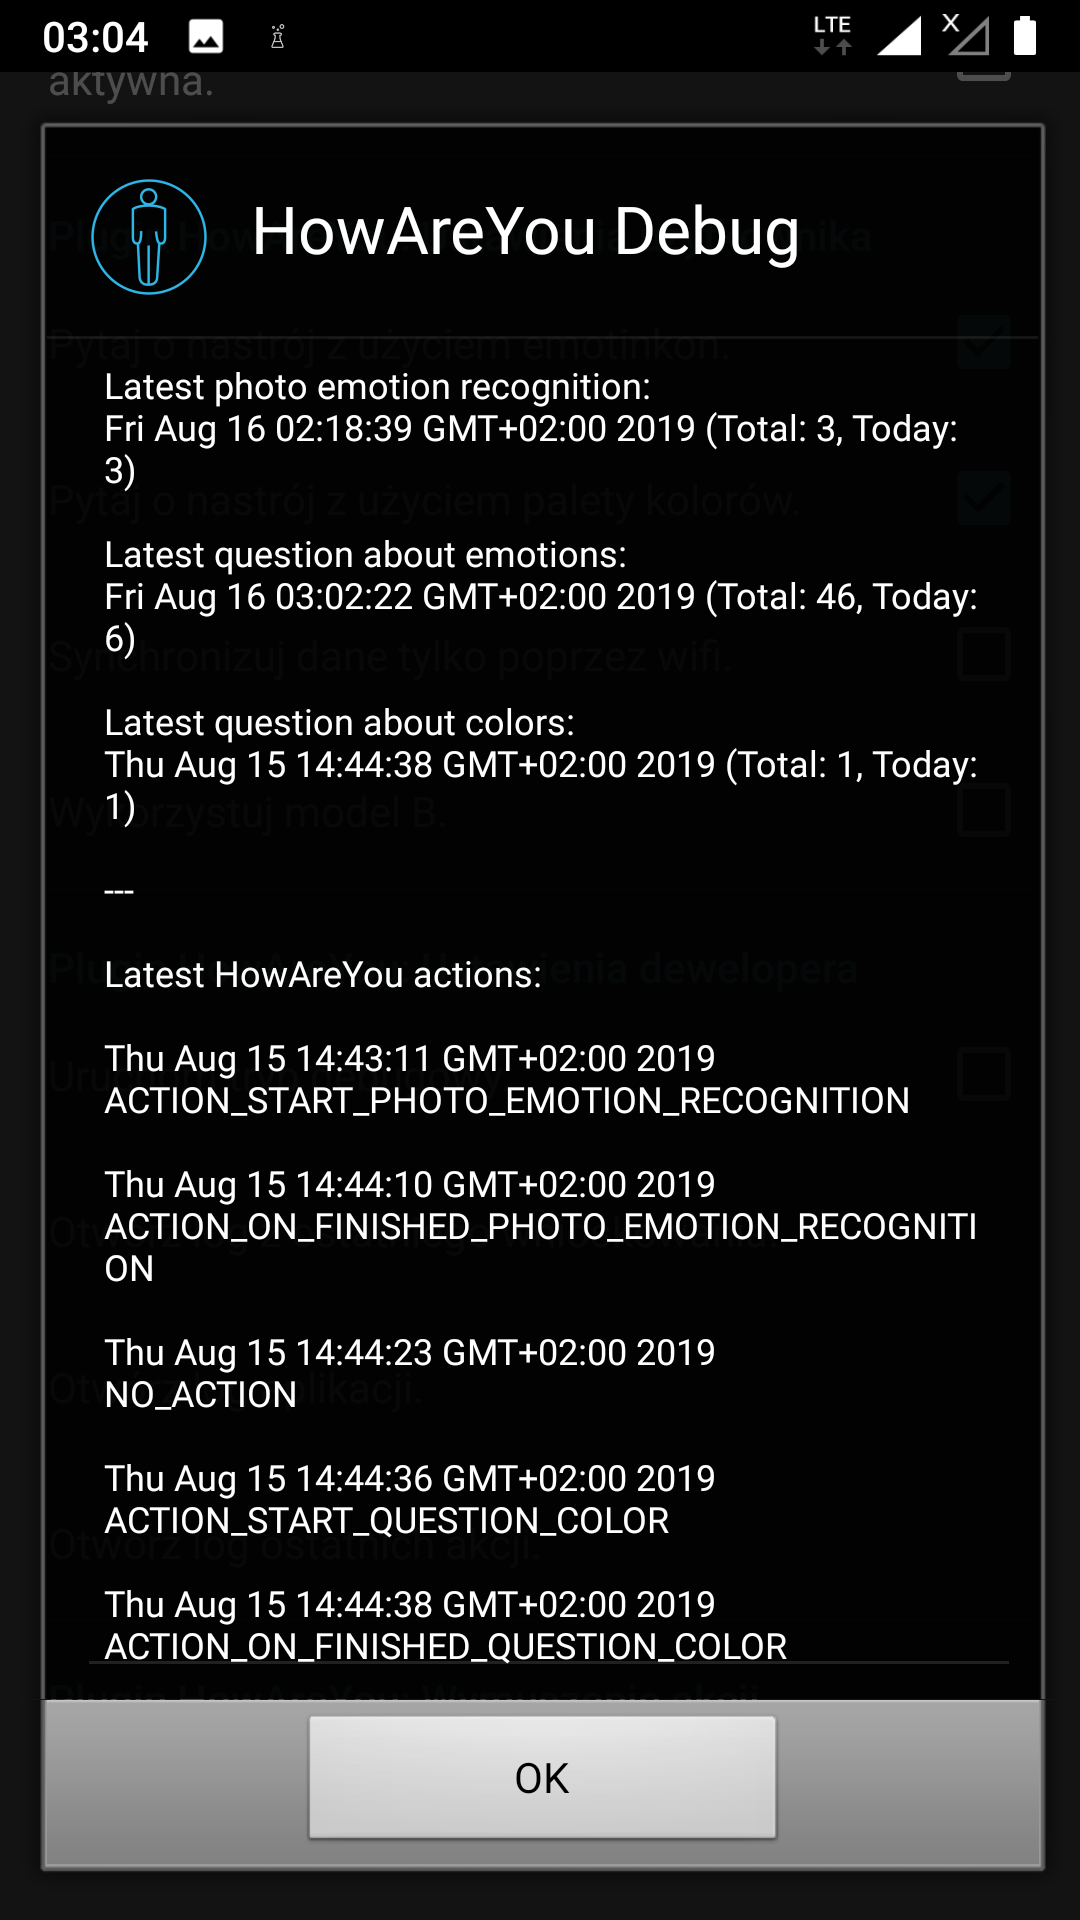
\includegraphics[scale=0.13]{rozdzial3/Ustawienia_logOstatnichAkcji.png}
		\subcaption{\label{subfigure_b}}
	\end{subfigure}
	\caption{ Log aplikacji \textit{HowAreYou} (a) oraz log ostatnich akcji (b).}
\end{figure}

Ostatnią z~możliwości menu Ustawień jest opcja wymuszenia. Ręcznie można wymusić zapytanie o kolor, zapytanie o emocje, czy skanowanie emocji z~wykorzystaniem kamery telefonu. Użytkownik może też wymusić synchronizację z~zewnętrzną bazą danych. Mimo, że sama synchronizacja uruchamiana jest przez plugin regularnie, wzięto pod uwagę, że może pojawić się sytuacja, kiedy synchronizacja jest potrzebna natychmiast, na przykład podczas krótkiej chwili połączenia z~siecią WiFi lub na zakończenie badania, aby nie stracić ostatnich wyników.



